\documentclass[journal,12pt,twocolumn]{IEEEtran}
%
\usepackage{setspace}
\usepackage{gensymb}
\usepackage{xcolor}
\usepackage{caption}
%\usepackage{subcaption}
%\doublespacing
\singlespacing

%\usepackage{graphicx}
%\usepackage{amssymb}
%\usepackage{relsize}
\usepackage[cmex10]{amsmath}
\usepackage{mathtools}
%\usepackage{amsthm}
%\interdisplaylinepenalty=2500
%\savesymbol{iint}
%\usepackage{txfonts}
%\restoresymbol{TXF}{iint}
%\usepackage{wasysym}
\usepackage{amsthm}
\usepackage{mathrsfs}
\usepackage{txfonts}
\usepackage{stfloats}
\usepackage{cite}
\usepackage{cases}
\usepackage{subfig}
%\usepackage{xtab}
\usepackage{longtable}
\usepackage{multirow}
%\usepackage{algorithm}
%\usepackage{algpseudocode}
\usepackage{enumitem}
\usepackage{mathtools}
%\usepackage{iithtlc}
%\usepackage[framemethod=tikz]{mdframed}
\usepackage{listings}
    \usepackage[latin1]{inputenc}                                 %%
    \usepackage{color}                                            %%
    \usepackage{array}                                            %%
    \usepackage{longtable}                                        %%
    \usepackage{calc}                                             %%
    \usepackage{multirow}                                         %%
    \usepackage{hhline}                                           %%
    \usepackage{ifthen}                                           %%
  %optionally (for landscape tables embedded in another document): %%
    \usepackage{lscape}     



%\usepackage{stmaryrd}


%\usepackage{wasysym}
%\newcounter{MYtempeqncnt}
\DeclareMathOperator*{\Res}{Res}
%\renewcommand{\baselinestretch}{2}
\renewcommand\thesection{\arabic{section}}
\renewcommand\thesubsection{\thesection.\arabic{subsection}}
\renewcommand\thesubsubsection{\thesubsection.\arabic{subsubsection}}

\renewcommand\thesectiondis{\arabic{section}}
\renewcommand\thesubsectiondis{\thesectiondis.\arabic{subsection}}
\renewcommand\thesubsubsectiondis{\thesubsectiondis.\arabic{subsubsection}}

% correct bad hyphenation here
\hyphenation{op-tical net-works semi-conduc-tor}

\lstset{
language=C,
frame=single, 
breaklines=true
}

%\lstset{
	%%basicstyle=\small\ttfamily\bfseries,
	%%numberstyle=\small\ttfamily,
	%language=Octave,
	%backgroundcolor=\color{white},
	%%frame=single,
	%%keywordstyle=\bfseries,
	%%breaklines=true,
	%%showstringspaces=false,
	%%xleftmargin=-10mm,
	%%aboveskip=-1mm,
	%%belowskip=0mm
%}

%\surroundwithmdframed[width=\columnwidth]{lstlisting}
\def\inputGnumericTable{}                                 %%
\lstset{
language=C,
frame=single, 
breaklines=true
}
 

\begin{document}
%

\theoremstyle{definition}
\newtheorem{theorem}{Theorem}[section]
\newtheorem{problem}{Problem}
\newtheorem{proposition}{Proposition}[section]
\newtheorem{lemma}{Lemma}[section]
\newtheorem{corollary}[theorem]{Corollary}
\newtheorem{example}{Example}[section]
\newtheorem{definition}{Definition}[section]
%\newtheorem{algorithm}{Algorithm}[section]
%\newtheorem{cor}{Corollary}
\newcommand{\BEQA}{\begin{eqnarray}}
\newcommand{\EEQA}{\end{eqnarray}}
\newcommand{\define}{\stackrel{\triangle}{=}}

\bibliographystyle{IEEEtran}
%\bibliographystyle{ieeetr}

\providecommand{\nCr}[2]{\,^{#1}C_{#2}} % nCr
\providecommand{\nPr}[2]{\,^{#1}P_{#2}} % nPr
\providecommand{\mbf}{\mathbf}
\providecommand{\pr}[1]{\ensuremath{\Pr\left(#1\right)}}
\providecommand{\qfunc}[1]{\ensuremath{Q\left(#1\right)}}
\providecommand{\sbrak}[1]{\ensuremath{{}\left[#1\right]}}
\providecommand{\lsbrak}[1]{\ensuremath{{}\left[#1\right.}}
\providecommand{\rsbrak}[1]{\ensuremath{{}\left.#1\right]}}
\providecommand{\brak}[1]{\ensuremath{\left(#1\right)}}
\providecommand{\lbrak}[1]{\ensuremath{\left(#1\right.}}
\providecommand{\rbrak}[1]{\ensuremath{\left.#1\right)}}
\providecommand{\cbrak}[1]{\ensuremath{\left\{#1\right\}}}
\providecommand{\lcbrak}[1]{\ensuremath{\left\{#1\right.}}
\providecommand{\rcbrak}[1]{\ensuremath{\left.#1\right\}}}
\theoremstyle{remark}
\newtheorem{rem}{Remark}
\newcommand{\sgn}{\mathop{\mathrm{sgn}}}
\providecommand{\abs}[1]{\left\vert#1\right\vert}
\providecommand{\res}[1]{\Res\displaylimits_{#1}} 
\providecommand{\norm}[1]{\lVert#1\rVert}
\providecommand{\mtx}[1]{\mathbf{#1}}
\providecommand{\mean}[1]{E\left[ #1 \right]}
\providecommand{\fourier}{\overset{\mathcal{F}}{ \rightleftharpoons}}
%\providecommand{\hilbert}{\overset{\mathcal{H}}{ \rightleftharpoons}}
\providecommand{\system}{\overset{\mathcal{H}}{ \longleftrightarrow}}
	%\newcommand{\solution}[2]{\textbf{Solution:}{#1}}
\newcommand{\solution}{\noindent \textbf{Solution: }}
\providecommand{\dec}[2]{\ensuremath{\overset{#1}{\underset{#2}{\gtrless}}}}
%\numberwithin{equation}{subsection}
\numberwithin{equation}{problem}
%\numberwithin{problem}{subsection}
%\numberwithin{definition}{subsection}
\makeatletter
\@addtoreset{figure}{problem}
\makeatother

\let\StandardTheFigure\thefigure
%\renewcommand{\thefigure}{\theproblem.\arabic{figure}}
%\renewcommand{\thefigure}{\theproblem}


%\numberwithin{figure}{subsection}

%\numberwithin{equation}{subsection}
%\numberwithin{equation}{section}
%%\numberwithin{equation}{problem}
%%\numberwithin{problem}{subsection}
%\numberwithin{problem}{section}
%%\numberwithin{definition}{subsection}
%\makeatletter
%\@addtoreset{figure}{problem}
%\makeatother
%\makeatletter
%\@addtoreset{table}{problem}
%\makeatother

%\let\StandardTheFigure\thefigure
\let\StandardTheTable\thetable
%\renewcommand{\thefigure}{\theproblem.\arabic{figure}}
%\renewcommand{\thefigure}{\theproblem}
\renewcommand{\thetable}{\theproblem}
%\numberwithin{figure}{section}

%%\numberwithin{figure}{subsection}



\def\putbox#1#2#3{\makebox[0in][l]{\makebox[#1][l]{}\raisebox{\baselineskip}[0in][0in]{\raisebox{#2}[0in][0in]{#3}}}}
     \def\rightbox#1{\makebox[0in][r]{#1}}
     \def\centbox#1{\makebox[0in]{#1}}
     \def\topbox#1{\raisebox{-\baselineskip}[0in][0in]{#1}}
     \def\midbox#1{\raisebox{-0.5\baselineskip}[0in][0in]{#1}}

\vspace{3cm}

\title{ Calculator using Wiring Pi and LCD}
%\title{
%	\logo{Matrix Analysis through Octave}{\begin{center}\includegraphics[scale=.24]{tlc}\end{center}}{}{HAMDSP}
%}


% paper title
% can use linebreaks \\ within to get better formatting as desired
%\title{Matrix Analysis through Octave}
%
%
% author names and IEEE memberships
% note positions of commas and nonbreaking spaces ( ~ ) LaTeX will not break
% a structure at a ~ so this keeps an author's name from being broken across
% two lines.
% use \thanks{} to gain access to the first footnote area
% a separate \thanks must be used for each paragraph as LaTeX2e's \thanks
% was not built to handle multiple paragraphs
%

\author{R Rohith Reddy$^{\dagger}$ and G V V Sharma$^{*}$ %<-this  stops a space
\thanks{*The author is with the Department
of Electrical Engineering, Indian Institute of Technology, Hyderabad
502285 India e-mail:  gadepall@iith.ac.in. $\dagger$ The author was an intern at IIT Hyderabad in the summer of 2017 e-mail:  rohithreddy0087@gmail.com}% <-this % stops a space
%\thanks{J. Doe and J. Doe are with Anonymous University.}% <-this % stops a space
%\thanks{Manuscript received April 19, 2005; revised January 11, 2007.}}
}
% note the % following the last \IEEEmembership and also \thanks - 
% these prevent an unwanted space from occurring between the last author name
% and the end of the author line. i.e., if you had this:
% 
% \author{....lastname \thanks{...} \thanks{...} }
%                     ^------------^------------^----Do not want these spaces!
%
% a space would be appended to the last name and could cause every name on that
% line to be shifted left slightly. This is one of those "LaTeX things". For
% instance, "\textbf{A} \textbf{B}" will typeset as "A B" not "AB". To get
% "AB" then you have to do: "\textbf{A}\textbf{B}"
% \thanks is no different in this regard, so shield the last } of each \thanks
% that ends a line with a % and do not let a space in before the next \thanks.
% Spaces after \IEEEmembership other than the last one are OK (and needed) as
% you are supposed to have spaces between the names. For what it is worth,
% this is a minor point as most people would not even notice if the said evil
% space somehow managed to creep in.



% The paper headers
%\markboth{Journal of \LaTeX\ Class Files,~Vol.~6, No.~1, January~2007}%
%{Shell \MakeLowercase{\textit{et al.}}: Bare Demo of IEEEtran.cls for Journals}
% The only time the second header will appear is for the odd numbered pages
% after the title page when using the twoside option.
% 
% *** Note that you probably will NOT want to include the author's ***
% *** name in the headers of peer review papers.                   ***
% You can use \ifCLASSOPTIONpeerreview for conditional compilation here if
% you desire.




% If you want to put a publisher's ID mark on the page you can do it like
% this:
%\IEEEpubid{0000--0000/00\$00.00~\copyright~2007 IEEE}
% Remember, if you use this you must call \IEEEpubidadjcol in the second
% column for its text to clear the IEEEpubid mark.



% make the title area
\maketitle

%\newpage

%\tableofcontents


%\begin{abstract}
%%\boldmath
%In this letter, an algorithm for evaluating the exact analytical bit error rate  (BER)  for the piecewise linear (PL) combiner for  multiple relays is presented. Previous results were available only for upto three relays. The algorithm is unique in the sense that  the actual mathematical expressions, that are prohibitively large, need not be explicitly obtained. The diversity gain due to multiple relays is shown through plots of the analytical BER, well supported by simulations. 
%
%\end{abstract}
% IEEEtran.cls defaults to using nonbold math in the Abstract.
% This preserves the distinction between vectors and scalars. However,
% if the journal you are submitting to favors bold math in the abstract,
% then you can use LaTeX's standard command \boldmath at the very start
% of the abstract to achieve this. Many IEEE journals frown on math
% in the abstract anyway.

% Note that keywords are not normally used for peerreview papers.
%\begin{IEEEkeywords}
%Cooperative diversity, decode and forward, piecewise linear
%\end{IEEEkeywords}



% For peer review papers, you can put extra information on the cover
% page as needed:
% \ifCLASSOPTIONpeerreview
% \begin{center} \bfseries EDICS Category: 3-BBND \end{center}
% \fi
%
% For peerreview papers, this IEEEtran command inserts a page break and
% creates the second title. It will be ignored for other modes.
\IEEEpeerreviewmaketitle


%\documentclass{article}
%\usepackage[utf8]{inputenc}
%\usepackage{listings}
%\usepackage{graphicx}

%\usepackage{color}
%\definecolor{codegreen}{rgb}{0,0.6,0}
%\definecolor{codegray}{rgb}{0.5,0.5,0.5}
%\definecolor{codepurple}{rgb}{0.58,0,0.82}
%\definecolor{backcolour}{rgb}{0.95,0.95,0.92}
%\lstdefinestyle{mystyle}{
    %backgroundcolor=\color{backcolour},   
    %commentstyle=\color{codegreen},
    %keywordstyle=\color{magenta},
    %numberstyle=\tiny\color{codegray},
    %stringstyle=\color{codepurple},
    %basicstyle=\footnotesize,
    %breakatwhitespace=false,         
    %breaklines=true,                 
    %captionpos=b,                    
    %keepspaces=true,                 
    %numbers=left,                    
    %numbersep=5pt,                  
    %showspaces=false,                
    %showstringspaces=false,
    %showtabs=false,                  
    %tabsize=2
%}
 
%\lstset{style=mystyle}
\section{Objective}
	To make a simple calculator using Raspberry Pi where input is given through keyboard and display the whole operation on a 16x2 LCD display.
\section{Components Required}
\begin{enumerate}
 	\item Resistor-220Ohm
 	\item Raspberry Pi
 	\item 16x2 LCD display
 	\item Jumper wires
\end{enumerate}

\section{Introduction}
	\subsection{Raspberry Pi}
		The Raspberry Pi is a low cost, credit-card sized computer that plugs into a computer monitor or TV, and uses a standard keyboard, mouse, power supply and a micro SD card with installed Linux Distribution. It is a capable little device that enables people of all ages to explore computing, and to learn how to program in languages like Scratch and Python.
	\begin{figure}[h]
	\centering
		\begin{minipage}[t]{.5\linewidth}
		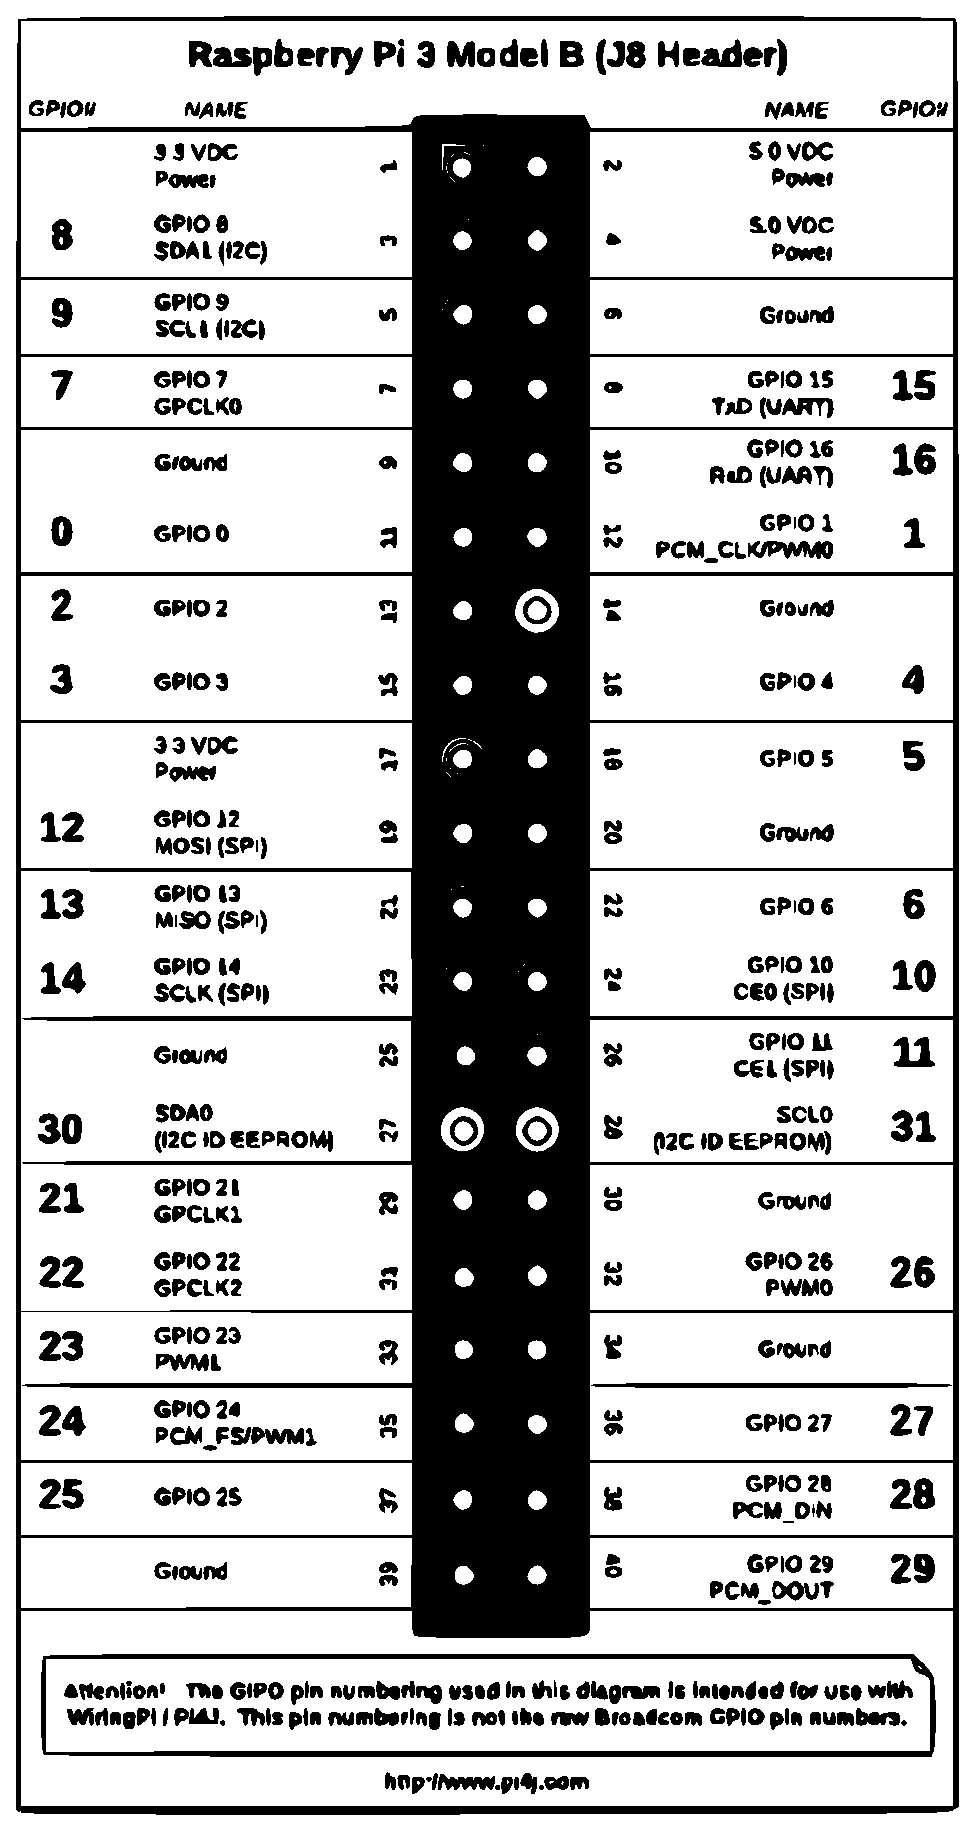
\includegraphics[scale=1]{rasp}
		\caption{ RPi 3B pin diagram}
		\label{fig:1}  
		\end{minipage}
	\end{figure}
	\subsection{16x2 LCD}
		LCD (Liquid Crystal Display) screen is an electronic display module and find a wide range of applications.A 16x2 LCD means it can display 16 characters per line and there are 2 such lines. In this LCD each character is displayed in 5x7 pixel matrix.

\section{Hardware Setup}
		
	\subsection{LCD to Raspberry Pi connections}
		\begin{enumerate}
		\item Connect the 5V pin i.e., pin 2 of the Raspberrry Pi to an extreme pin of the Breadboard. Let this pin be Vcc.
		\item Connect the GND pin i.e., pin 6 of the Pi to the opposite extreme pin of the Breadboard.
		\item Plug the LCD in Figure 1 to the bread-board.
		\item  Connect the 220$\Omega$ resistance from Vcc to pin 15 (Led+) of the LCD.
		\item Connect the raspberry pi pins to the LCD display as shown in the table below.
		\end{enumerate}
\begin{figure}


\begin{minipage}[h]{.5\linewidth}
		\centering
		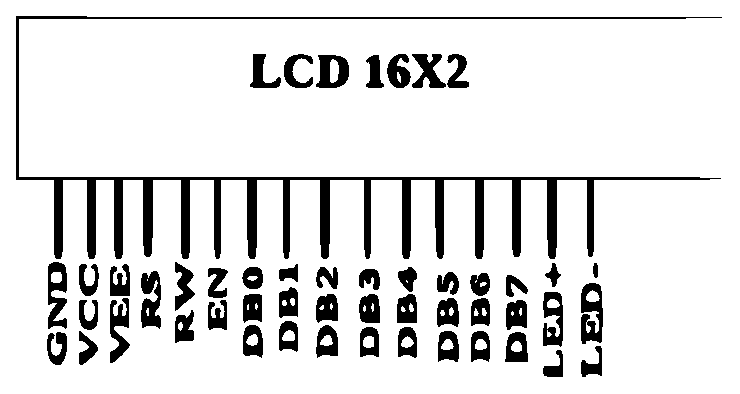
\includegraphics[scale=1.2]{lcd}
	    \caption{LCD pin out}
		\label{fig:1}
	\end{minipage}
\end{figure}
	\begin{table}[h]
	\centering
		\begin{minipage}[b]{0.56\linewidth}
			\centering
			\begin{tabular}{ |c|c| }
			\hline
			LCD pins & Raspberry Pi pins\\
			\hline
			GND & Ground\\
			Vcc & 5V\\
			Vss & Ground\\
			RS  & GPIO 25\\
			R/W & Ground\\
			EN  & GPIO 24\\
			DB4 & GPIO 23\\
			DB5 & GPIO 22\\
			DB6 & GPIO 21\\
			DB7 & GPIO 14\\
			LED+ & 5V\\
			LED- & Ground\\
			\hline
			\end{tabular}
			\caption{Raspberry Pi to LCD connections}
			\label{Table}			
	\end{minipage}	
	
		
\end{table}
\section{Software Setup}
The following commands will install wiring pi module.\\

\fbox{\begin{minipage}{19em}\
 	sudo apt-get install git-core\\
 	sudo apt-get update sudo apt-get upgrade\\
 	cd git clone git ://git.drogon.net/wiringPi\\
 	cd  ~/wiringPi\\
 	./build 
 	
\end{minipage}}\\\

\section{Programming of Raspberry Pi}
\begin{enumerate}
	\item The code is written in C language by importing the wiring Pi library.
	\item WiringPi is a PIN based GPIO access library written in C for the BCM2835, BCM2836 and BCM2837 SoC devices used in all Raspberry Pi.
	\item Save the following code in a file called calculatorpi .\\
	\\
		\fbox{\begin{minipage}{19em}
https://github.com/rohithreddy0087/Calculator-using-Raspberry-Pi/blob/master/codes./C code
\end{minipage}}\\
	\item Run the program using following command.\\
	\\
	\fbox{\begin{minipage}{19em}
 	gcc -o calculatorpi calculatorpi.c -lwiringPi -lwiringPiDev
\end{minipage}}\\
	\end{enumerate}

\section{Specifications of Calculator}
\begin{enumerate}

	\item Any number of inputs can be given to the calculator with any operations between the operands.
	\item The input can be a decimal number also and  can be a n digit number.
	\item If more than two inputs is given,it performs calculation of first two operands and the obtained result is used for next calculation with third operand and so on.\\
	For example if 2+3*4 is given it first adds 2+3=5 and this 5 is multiplied to 4 and the final result will be shown as 20.
	\item The result of the given input calculation along with the calculation entered is displayed on the LCD display for 4s.After 4s we can enter new calculation.
			
\end{enumerate}

\section{Conclusions}
A simple calculator with basic operations is made using a Raspberry Pi.GPIO pins of the Pi are used in making the hardware interface with the LCD.\\
Using C programming and wiring Pi,we can write code for the calculator by importing necessary libraries.
\end{document}


